\documentclass[../main.tex]{subfiles}
\begin{document}
Inferring topics from the words in a document is a crucial task in many natural language processing tasks.
The noisy-or topic model\cite{liu2016representing} is one such example, which is quite simple yet effective.
It is a Bayesian network consisting of two types of nodes; one type are the domain keyphrases (topics) that are latent while others are the content units (words) which are observed.
Words have only topics as their parents. To capture hierachical nature of topics, they can have other topics as parents.
See figure \ref{fig:fig3} which illustrates the model structure. \newline
\begin{figure}[h]
  \centering
  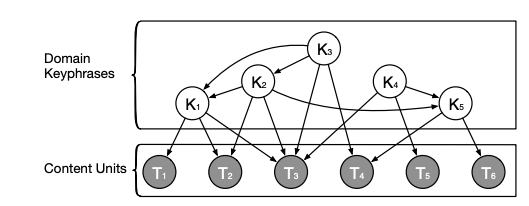
\includegraphics[width=100mm]{overview_noisy_or_topic.png}
  \caption{Illustrative Bayesian network for the Noisy-Or Topic model\cite{liu2016representing}}
  \label{fig:fig3}
\end{figure}

Let $Z$ be the the set of all nodes in the network.
Each model has a leak node $O$ which is the parent of all other nodes.
The set of keyphrases is denoted by $K$ and the set of content units is represented as $T$.
The number of children for each keyphrase $K_i$ is sampled from a poisson prior:
$$
|Children(K_i)| \sim Poisson(\lambda_{fanout})
$$
The children are chosen at random without replacement from the rest of the nodes in $Z \in [i+1,|Z|]$
. The weight of the leak node $O$ to all the nodes ($W_{oj}$) is sampled from an exponential prior:
$$
W_{oj} \sim Exponential(scale_{leak weight})
$$
The weight of keyphrase node $K_i$ for child $j$ is sampled from an exponential prior:
$$
W_{ij} \sim Exponential(scale_{weight})
$$
The likelihood for each node $j$ in $Z$ is given as:
$$
P(Z_j|Parents(Z_j)) = 1 - \exp(-W_{oj} -\sum_{i}(W_{ij} * Z_i))
$$
and the state of each node $j$ in $Z$ is sampled from a Bernoulli distribution with the above probability:
$$
Z_j \sim Bernoulli(P(Z_j|Parents(Z_j)))
$$
\subsection{Data Generation}
For the experiment, we first sample the model structure.
This consists of determining the parent key-phrase nodes for each content units, as well as which key-phrase nodes are parent of each key-phrase node.
Next, the weights are sampled for all connections from thier respective priors.
The hyperprior configuration is listed in table \ref{tab:table_NOT}.
Now the key-phrase nodes are sampled once; and two instances of content units are sampled keeping the key-phrase nodes fixed.
One instance is passed to PPL implementation for inference, while the other is used to compute posterior predictive of the obtained samples.
\begin{table}[h]
 \caption{Hyperpriors for Noisy-Or Topic Model}
  \centering
  \begin{tabular}{lll}              \\
    \cmidrule(r){1-3}
    Hyperprior             & Value         & Notes  \\
    \midrule
    $\lambda_{fanout}$     & 3             & Poisson prior for number of children to each key-phrase node  \\
    $scale_{leak weight}$  & 0.1           & Exponential prior for $W_{oj}$ \\
    $scale_{weight}$       & 1             & Exponential prior for $W_{ij}$ \\
    word fraction          & $\frac{2}{3}$ & ratio of number of content units to all nodes \\
    \bottomrule
  \end{tabular}
  \label{tab:table_NOT}
\end{table}
\subsection{PPL Implementations}
The model was implemented in Stan and Jags PPLs, with the help of PyStan\cite{PyStan} and PyJAGS\cite{PyJAGS} libraries for interface.
The compilation and inference times were recorded.
The model requires the support for discrete latent variables, which JAGS has, but Stan does not.
This means that the Stan implementation requires a reparameterization for denoting whether a node is activated or not.
This was achieved representing boolean variables as a relaxation of 1-hot encoded vectors\cite{maddison2016concrete}.
So, for example, if true is represented by $[1, 0]$ and false by $[0, 1]$ in the 1-hot encoding then a relaxed representation of a true value might look like [0.9999, 0.0001].
The reparameterization process is as follows:
First, you encode the probabilities of a node in paramter vector $\alpha = [\alpha_{true}, \alpha_{false}]$:

$$
\alpha_{true} = P(Z_j|Parents(Z_j)), \quad \alpha_{false} = 1 - P(Z_j|Parents(Z_j))
$$
We choose a temprature parameter $\tau = 0.1$.
Then for each keyphrase, you assign an intermedieate random variable $X_j$:
$$
X_j = softmax(\log\alpha_j + G_j/\tau), \quad Where, G_j \stackrel{iid}{\sim} Gumbel(0,1)
$$
We then obtain $Z_j$ from $X_j$ as follows:
$$
Z_j = 1 - argmax(X_j)
$$
\begin{figure}[h]
  \centering
  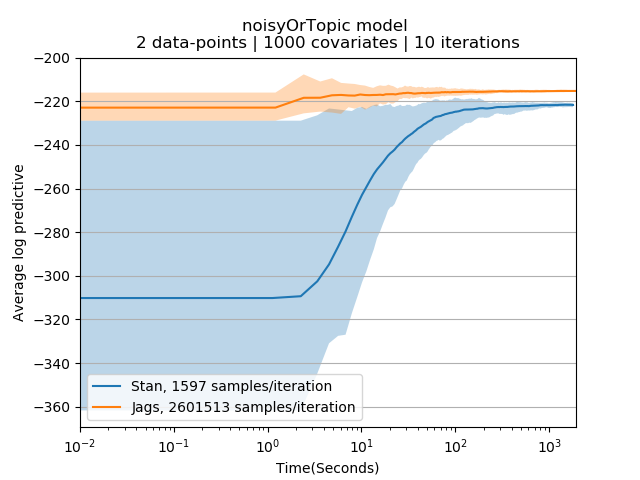
\includegraphics[width=150mm]{analysis_noisy_or_topic.png}
  \caption{Posterior convergence behaviour of Jags and Stan for Crowdsourced Annotation Model}
  \label{fig:fig2}
\end{figure}

\subsection{Results}
Figure \ref{fig:fig2} shows the comparative performance.
From the figure, we can make the following observations:
\begin{itemize}
\item JAGS converges to higher log-likelihood than Stan, this can be due to the reparameterization of Stan.
\item JAGS is both faster to converge as well has a much lower time per sample.
\item JAGS' inference starts sampling from relatively high log-likelihood space  and hence converges much quicker than STAN's, which can again be attributed to the reparameterization.
\end{itemize}
\end{document}
